\documentclass[12pt]{article}

\usepackage{sbc-template}

\usepackage{float}

\usepackage{graphicx,url}

%\usepackage[brazil]{babel}   
\usepackage[utf8]{inputenc}  

     
\sloppy

\title{APLICAÇÃO WEB DISTRIBUÍDA PARA MAPEAMENTO DE DESCASOS PÚBLICOS: UM ESTUDO DE CASO NA CIDADE DE FLORIANO-PI.}

\author{Anderson F. Santos, Kléssiton R. Silva, Romário C. Oliveira}

\address{Instituto de Informática -- Universidade Federal do Piauí
  (IFPI)\\
  Caixa Postal 15.064 -- 91.501-970 -- Piauí -- PI -- Brasil
\nextinstitute
  Departamento de Sistemas e Computação\\
  Universidade Regional de Blumenal (FURB) -- Blumenau, SC -- Brazil
  \email{\{nedel,flavio\}@inf.ufrgs.br, R.Bordini@durham.ac.uk,
  jomi@inf.furb.br}
}

\begin{document} 

\maketitle

\begin{abstract}


\end{abstract}
     
\begin{resumo} 
  
  
\end{resumo}

\section{Introdução}
Com a constante evolução das tecnologias nos mais variados ramos, desde a manipulação genética até a transmissão de informações, onde a tecnologia trabalhando em conjunto com a informação tem  demonstrado não só o seu potencial, mas também se situa como alimento de diversas ideologias ambiciosas concebidas para o futuro da nossa civilização. Uma dessas ideologias direcionadas ao nosso bem como sociedade está às chamadas Tecnologias de informação e comunicação (TIC’s) que em termos gerais pode ser entendida com um conjunto de recursos tecnológicos, utilizados de forma integrada para um objetivo em comum, tendo esse conceito em mente, às TIC’s são uma ideia que tem se tornado cada vez mais abrangente como um meio de comunicação, tendo como exemplo do potencial das TIC’s podemos levar em conta as Redes Sociais que se tornaram um meio massivo de comunicação e propagação de ideias.

Olhando para tal potencial apresentado, as TIC’s têm se propagado pelo setor governamental, trazendo a tona uma proposta de governo eletrônico, caracterizado pela informatização de suas tarefas internas e pela estabilidade da comunicabilidade com o público externo: cidadãos, fornecedores, empresas etc. , visando o aumento e participação da sociedade nas ações administrativas do seu município (GOMES, 2008). E essa otimização na prestação de serviços, em conjunto do fortalecimento da relação entre cidadãos e administração pública, se faz cada vez mais necessários, uma vez que os órgãos governamentais vem sendo constantemente desafiados a promover políticas de gestão públicas efetivas e transparentes.

É através deste cenário que aplicações e sistemas digitais surgem como importantes ferramentas de apoio e suporte a gestão pública, deixando de lado o velho modo “Esperar até que governo faça algo a respeito!’’, para tomar como fundamento base o engajamento da própria sociedade como entidade fiscalizadora e cabendo a administração pública a tarefa de ouvir e atender a essa necessidade. Tais aplicações atuam como um elo interativo entre o poder público e a população geral, sendo classificadas como sistema colaborativos (MAGALHÃES, 2015) e segundo Gugliano (2015) esses processos participativos têm produzido novas redes e novas interações entre grupos sociais e atores estatais, revelando diferentes graus de institucionalização de acordo com o nível de governo e a dinâmica política no interior de cada setor de política pública.

Portanto, este presente projeto, foi realizado com o objetivos de desenvolver uma aplicação web/mobile para o mapeamento de pontos de descasos públicos na cidade de Floriano Piauí. Visando, contribuir para uma atuação mais participativa da população e melhor gestão administrativa do município.

\section{Objetivos}
\subsection{Objetivo geral}
Mapear pontos de descasos públicos na cidade de Floriano Piauí para auxiliar na tomada de decisão pela prefeitura, por meio de uma aplicação Web mobile.
\subsection{Objetivos específicos}
\begin{itemize}
\item Desenvolver uma aplicação Web mobile para mapear denúncias relacionadas aos pontos de descasos públicos.
\item Identificar e mapear pontos de descasos públicos da cidade de Floriano Piauí.
\item Disponibilizar os dados gerados ao longo do mapeamento para auxiliar a\\ prefeitura de Floriano Piauí na identificação de falhas na prestação de serviços.
\end{itemize}

\section{Justificativa}
A Constituição Federal 1988 atribuiu ao Poder Público a responsabilidade da prestação de serviços públicos à sociedade, definido que tal atividade poderá ser realizada de forma direta (através do próprio Estado) ou indireta (através do particular). Portanto, a administração pública deve atender as necessidades básicas coletivas das sociedades. Dentre todos os serviços prestados pela Administração Pública, aquele mais importante é o chamado serviço público essencial, que são àqueles serviços ou atividades indispensáveis à sobrevivência do ser humano. Estão eles dispostos no artigo 10 da Lei 7783/89:
\\Art. 10 São considerados serviços ou atividades essenciais:
\\I - Tratamento e abastecimento de água; produção e distribuição de energia elétrica, gás e combustíveis;    
\\II - Assistência médica e hospitalar;
\\III - distribuição e comercialização de medicamentos e alimentos;
\\IV - Funerários;
\\V - Transporte coletivo;
\\VI - Captação e tratamento de esgoto e lixo;
\\VII - telecomunicações;
\\VIII - guarda, uso e controle de substâncias radioativas, equipamentos e materiais nucleares;
\\IX - Processamento de dados ligados a serviços essenciais;
\\X - Controle de tráfego aéreo;
\\XI - compensação bancária.

No entanto, a população brasileira vem sofrendo com o grande número de descasos públicos, gerando uma enorme insatisfação, instigada pelo fato do país possuir uma das mais altas cargas tributárias do mundo, não sendo convertida em prestação de serviços de qualidade em mesma escala. Tal problema vem se arrastando ao longo do tempo, sendo alimentado por gestões públicas oclusas, e nas últimas décadas, a sociedade brasileira se mostrou bastante interessada na construção de um modelo de gestão pública mais receptível às necessidades dos cidadãos e mais eficiente na prestação dos serviços públicos (ROBERTO, 2007). Uma das alternativas encontradas foi promover a participação popular na administração pública, por meio do uso das TICs, isso implica na ampliação do espaço público, no reconhecimento de novos atores coletivos e de uma nova lógica de participação social.

Esse movimento foi impulsionado principalmente por um aumento considerável na utilização das novas TICs pela sociedade e a migração da informação baseada em papel para mídias digitais (DINIZ et al., 2009). O uso das novas TICs visa ampliar a participação cidadã nas tomadas de decisões da gestão pública, promovendo a colaboração popular no processo democrático de tomada de decisão. Utilizando essas tecnologias, pode-se conseguir um forte controle sobre o aparelho burocrático, ao gerir melhor a informação, e como este processo pode resultar em impactos positivos na sociedade, entre eles, o diminuir os níveis de ineficiência, de corrupção e aumento da transparência.

Ou seja, as TICs possuem um grande potencial democrático, desde que haja delimitação política no caminho da participação popular e da transparência, pois o governo pode ter dificuldades em disponibilizar determinadas informações, manter sistemas consistentes e interativos. É notória a importância da participação da sociedade na gestão pública, sendo necessário o aperfeiçoamento dos mecanismos de funcionamento e ao alargamento dos seus espaços públicos de informação e comunicação.

\section{Referencial Teórico}
O aumento na utilização das novas tecnologias da informação e da comunicação (TICs) pela sociedade e a migração da informação baseada em papel para mídias eletrônicas (DINIZ et al., 2009) têm proporcionado uma manipulação mais eficiente e transparente das informações, oferecendo novas formas de interação entre as pessoas. Essa massiva utilização por parte da população também vem impulsionando muitas instituições governamentais a oferecerem novos canais de comunicação para a sociedade, visando interagir com os seus cidadãos. Logo após o surgimento da Web 2.0, termo cunhado em 2005 para se referir a uma nova geração de tecnologias que permite uma comunicação com maior nível de interatividade e colaboração através da Internet, oferecendo recursos e serviços para aplicações online e multimídia (BRESSAN, 2007). Nasceram muitas ferramentas de participação e colaboração eletrônica, também chamadas de plataformas de e-participação e de e-colaboração.

De acordo com Macintosh (2004), o termo e-participação, do inglês, e-participation, é constituída pelo elemento ― e, de eletrônico e tem uma associação com os termos  e-government e e-governance, que juntos, referem-se o uso das novas TICs visando ampliar a participação cidadã nas tomadas de decisões da administração pública, promovendo a participação popular no processo democrático de tomada de decisão, de forma eletrônica.

Sabendo que o incremento do número de iniciativas de e-participação tem despertado na academia o interesse em compreender as suas possibilidades e limites para promover e aprofundar o alcance da democracia participativa. Diversos autores destacam o potencial da internet para enfrentar o dilema de ampliar a participação dos cidadãos e o sentimento de pertencimento na vida política que afeta as democracias representativas liberais contemporâneas, pois tornaria a participação mais fácil, ágil e conveniente (GOMES, 2005).

Uma das soluções desenvolvidas nesse intuito, é a plataforma online COLAB que exerce o trabalho intermediate de comunicação entre Sociedade e Administração pública, e para entendermos como esse processo funciona na prática, podemos tomar como exemplo um caso hipotético de que uma pessoa ao percorrer por uma rua se depara com um encanamento quebrado ou o acúmulo de lixo em uma determinada local, diferentemente do que ocorre casualmente, onde a população espera o órgão responsável tomar a iniciativa de solucionar o problema, permitindo que o problema aumente gradativamente, por meio da aplicação é possível notificar a prefeitura sobre o problema, com imagens e a localização, para assim agilizar a solução daquela ocorrência.

O Brasil adota um regime político democrático, modelo de governo que vem sofrendo sinais de desgaste (FREITAS, 2015). Mas com o surgimento e aprimoramento da Internet e a evolução das TICs, passam a existir novos meios que visam promover uma sociedade mais democrática e participativa, através da participação e colaboração eletrônica ou e-participation e e-collaboration. Através destas plataformas, o cidadão pode fiscalizar, discutir, sugerir, reclamar, expor suas ideias e até se disponibilizar para resolver alguns problemas. Por isso o governo brasileiro também vem investindo na criação de novos mecanismos para ampliar os meios de participação eletrônica dos cidadãos, com o intuito de incluí-los no processo democrático, objetivando ouvir seus anseios e opiniões sobre diversas temáticas (FREIRE et al., 2011).

\section{Metodologia}\label{sec:figs}
\begin{figure}[H]
\centering
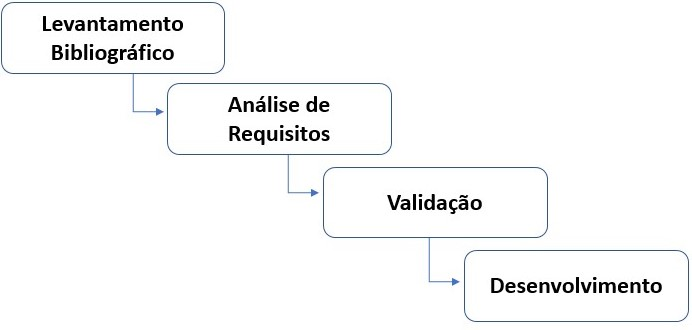
\includegraphics[width=15cm]{fig01.jpg}
\caption{Metodologia}
\end{figure}



\subsection{Levantamento Bibliográfico}
\subsection{Análise de Requisitos}
\subsection{Desenvolvimento}
\subsection{Validação}

\section{Conclusão e Resultados}\label{sec:figs}

\section{Cronograma}\label{sec:figs}


\bibliographystyle{sbc}
\bibliography{sbc-template}

\end{document}
